\documentclass{article}
\usepackage{tikz}
\usepackage{amsmath}
\usepackage{geometry}
\geometry{a4paper, margin=2cm}

\begin{document}

\section*{Symbolische Darstellung der Beta-Korrekturfrequenz}

\subsection*{Beta-Korrektur als fundamentale Frequenz}

Die aus der Optimierung der Beta-Skala resultierende Korrekturfrequenz

\[
\varepsilon = 0{,}000012151 \approx \frac{1}{8217} \approx \frac{4}{32901}
\]

kann mit hoher Präzision durch rationale Approximationen beschrieben werden.

\subsection*{Geometrischer Bezug: Einheitskreis in 33 Sektoren}

\begin{center}
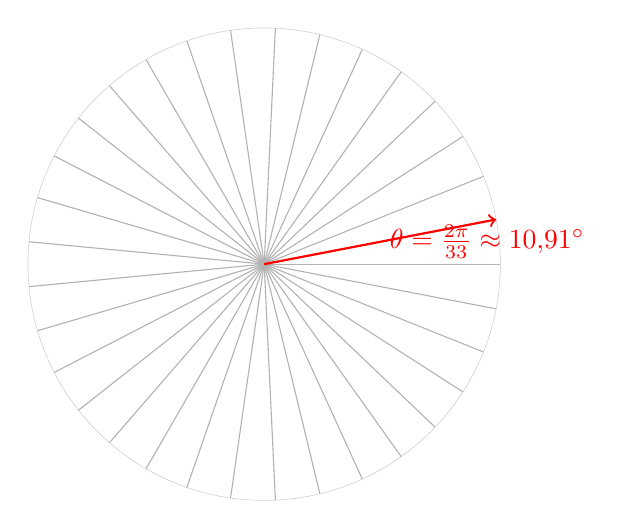
\begin{tikzpicture}[scale=3]
  \draw[very thin, gray!40] (0,0) circle(1cm);
  \foreach \i in {1,...,33} {
    \draw[gray!60, thin] (0,0) -- ({cos(360/33*\i)}, {sin(360/33*\i)});
  }
  \draw[red, thick, ->] (0,0) -- ({cos(360/33)}, {sin(360/33)});
  \node[red, right] at ({0.5*cos(360/33)}, {0.5*sin(360/33)}) 
    {$\theta = \frac{2\pi}{33} \approx 10{,}91^\circ$};
\end{tikzpicture}
\end{center}

\subsection*{Interpretation}
\begin{itemize}
  \item $33$: Zahl der Spiralwindungen pro DNA-Helixumdrehung
  \item Die Beta-Korrekturfrequenz $\varepsilon$ spiegelt mögliche periodische Resonanzen wider
\end{itemize}

\textbf{Bezeichnungsvorschlag:} \emph{Freese-Beta-Korrekturfrequenz} oder \emph{Fundamentale Skalenresonanz der Beta-Skala}

\end{document}